% !TeX root = main.tex
\section{A Second Example: Another Barcode}

Let us now consider the Hamiltonian diffeomorphism $\phi^2$, where $\phi$ is the diffeomorphism considered in the previous section, i.e.
\begin{equation}
\phi(x,y) = ( x + a \sin(y + a \sin(x)), y + a \sin(x)).
\end{equation}

The Hamiltonian diffeomorphism $\phi$ is the time $2a$ flow of the Hamiltonian $H_1$, defined in $\interval 0 {2a}$. Consequently, $\phi^2$ is the time $4a$ flow of the same Hamiltonian, now extended by periodicity to the interval $\interval 0 {2a}$. Slightly abusing notation, we will write $H_1$ for this extension. A similar observation applies to $H_0$.

We begin by computing the contractible $2a$-periodic orbits of $H_1$ in the torus, i.e. the solutions of $\phi^2(x,y) = (x,y)$ in $\R^2$.

\subsection{The Contractible Periodic Orbits}

\begin{prop}\label{prop:orbitsphi2}
If $a \leq 2$, the solutions to the equation $\phi^2(x,y) = (x,y)$ coincide with the solutions of $\phi(x,y) = (x,y)$, i.e. $(x,y) \in \pi \Z \times \pi \Z$.

If $2 < a < \pi$, there are four new solutions modulo $2\pi$. Let $(x_0, y_0)$ be the unique solution in $\ointerval 0 \pi \times \ointerval 0 \pi$. Then, the other three solutions are given by rotations of this solution about the origin, i.e.
\begin{equation}
(x_0, y_0), (-y_0, x_0), (-x_0, -y_0), \text{ and } (y_0, -x_0).
\end{equation}

Furthermore, $y_0 = \pi - x_0$, and $x_0$ is defined as the unique positive fixed point of $x \mapsto \frac a 2 \sin(x)$.
\end{prop}

\begin{proof}
We begin by writing out the equation $\phi^2(x,y) = (x,y)$ in full:
\begin{equation}\label{phi2id1}
\begin{gathered}
\begin{cases}
x + a \sin(y + a \sin(x)) + a \sin(y_2) = x,\\
y_2 = y,
\end{cases}\\
\text{Where $y_2 = y + a \sin(x) + a \sin(x + a \sin(y + a \sin(x)))$.}
\end{gathered}
\end{equation}

A few elementary computations will show that, for $a > 0$, equation \eqref{phi2id1} is equivalent to
\begin{equation}\label{phi2id2}
\begin{cases}
\sin(y + a \sin(x)) + \sin(y) = 0,\\
\sin(x - a \sin(y)) + \sin(x) = 0.
\end{cases}
\end{equation}

Now, recall that an equation of the form $\sin(A) = - \sin(B)$ has two types of solutions:
\begin{equation}
\begin{aligned}
A &= - B + 2 k \pi, \; k \in \Z && \text{(Type 1)}\\
A &= \pi + B + 2 k \pi, \; k \in \Z && \text{(Type 2).}
\end{aligned}
\end{equation}

Now, the restriction $a < \pi$ implies that neither of the equations in \eqref{phi2id2} has solutions of type 2. For example, a type 2 solution of the first equation would satisfy
\begin{equation}
y + a \sin(x) = \pi + y + 2 k \pi \iff a \sin(x) = \pi + 2 k \pi,
\end{equation}
which is impossible because the left-hand side is always less than $\pi$ in absolute value, while the right-hand side is always greater than or equal to $\pi$ in absolute value.

Therefore, the system \eqref{phi2id2} reduces to
\begin{equation}
\begin{cases}
y = - \frac a 2 \sin(x) + k_1 \pi,\\
x = \frac a 2 \sin(y) + k_2 \pi.
\end{cases}
\end{equation}

Modulo $2\pi$, there are only two cases, $(k_1, k_2) \in \{0,1\} \times \{0,1\}$.

We begin by showing that if $k_1 = k_2$ then there are only the trivial solutions $x = y = k_1 \pi$.

\begin{lemma}
For $k = 0, 1$ and $0 < a < \pi$, the system of equations
\begin{equation}
\begin{cases}
y = - \frac a 2 \sin(x) + k \pi,\\
x = \frac a 2 \sin(y) + k \pi,
\end{cases}
\end{equation}
has only the trivial solution $x = y = k \pi$.
\end{lemma}

\begin{lemmaproof}
It suffices to consider the case $k = 0$, as the other case can be reduced to this one via a change of variables. Suppose then that
\begin{equation}
\begin{cases}
y = - \frac a 2 \sin(x),\\
x = \frac a 2 \sin(y).
\end{cases}
\end{equation}

In this case, $x = - \frac a 2 \sin\left(\frac a 2 \sin(x)\right)$. Such a solution must satisfy $\abs x \leq \frac a 2 < \frac \pi 2$, and therefore the sign of $\sin(x)$ coincides with the sign of $x$. For the same reason $(\abs{\frac a 2 \sin(x)} \leq \frac a 2 < \frac \pi 2)$, the sign of $\sin\left(\frac a 2 \sin(x) \right)$ coincides with the sign of $\frac a2 \sin(x)$, which coincides with the sign of $x$. Unless $x=0$, this is an obvious contradiction.
\end{lemmaproof}

We now handle the case $k_1 \neq k_2$.

\begin{lemma}
For $k = 0, 1$ and $0 < a \leq 2$, the system of equations
\begin{equation}\label{phi2id3}
\begin{cases}
y = - \frac a 2 \sin(x) + k \pi,\\
x = \frac a 2 \sin(y) + (1-k) \pi,
\end{cases}
\end{equation}
has only the trivial solution $x = y = k \pi$.

On the other hand, if $2 < a < \pi$, there exist two new solutions for each value of $k$. The solutions $(x,y)$ to the case $k=0$ are in bijection with the solutions to the case $k=1$, via the map
\begin{equation}
(x,y) \mapsto (y, 2\pi - x).
\end{equation}

Furthermore, if $(x_0, y_0)$ is the unique solution to the $k=0$ case with $x_0 > 0$, we have $y_0 = \pi - x_0$. Finally, the three solutions to the $k_0$ case are $(-x_0, -y_0)$, $(0,0)$ and $(x_0, y_0)$.
\end{lemma}

\begin{lemmaproof}
The bijection between the solutions of the $k=0$ and $k=1$ cases holds regardless of the value of $a$, so both for $0<a\leq 2$ and for $2<a<\pi$ it suffices to verify the case $k=1$.

To find solutions of \eqref{phi2id3} for $k=1$, consider the map
\begin{equation}
\eta(x) = \frac a 2 \sin(x).
\end{equation}

Then, solutions of \eqref{phi2id3} are in one-to-one correspondence with fixed points of $\eta^2 = \eta \circ \eta$, so it suffices to consider that problem instead. Furthermore, since $\eta$ is odd, and consequently so is $\eta^2$, it suffices to look for positive solutions, which must obviously be in the interval $\linterval 0 {\frac a 2}$. Here are some facts about $\eta$ and $\eta^2$, which can be deduced by elementary calculus.
\begin{itemize}
\item The derivatives of $\eta$ and $\eta^2$ at zero are given by $\frac a 2$ and $\left( \frac a 2 \right)^2$ respectively,
\item Both of these functions are concave in $\interval 0 {\frac a 2}$, because their second derivative is negative (strictly except at zero),
\item Both of these functions are increasing in the interval $\interval 0 {\frac a 2}$. This uses the fact that $a < \pi$.	
\end{itemize}

The case $a < 2$ is now easy to solve, as in this event the derivative of $\eta^2(x) - x$ is negative at zero and decreasing in $\interval 0 {\frac a 2}$. Therefore, $\eta^2(x) - x$ is a decreasing function, and since it takes the value $0$ at $x = 0$, it cannot be zero again in the interval.

The case $a = 2$ is similar, though not as direct because the derivative of $\eta^2(x) - x$ at zero is now zero, instead of negative. However, by concavity, this function is still strictly decreasing in $\interval 0 {\frac a 2}$ and the same argument goes through.

Finally, we consider $2 < a < \pi$. In this case, the derivative of $\eta(x) - x$ is positive at zero, and therefore, for small enough values of $x$, $\eta(x) > x$. On the other hand, since $\abs{\eta(x)} \leq \frac a 2$ for all $x$, obviously $\eta(\frac a 2) \leq \frac a 2$. Therefore, by continuity, we have established the existence of a fixed point of $\eta$ in $\linterval 0 {\frac a 2}$, and consequently of a fixed point of $\eta^2$.

We now show that such a fixed point is unique. Since $\eta^2(x)$ is concave in the interval, so is $\eta^2(x) - x$. It is a known fact that a strictly concave function on an interval attains each value at most twice, and so in particular has at most two roots. One of the roots is $x = 0$, and the other is the root which we have proven exists. We call this root $x_0$. To it is associated a solution $(x_0, y_0)$ of \eqref{phi2id3}, satisfying $y_0 = \pi - \eta(x_0)$ and $x_0 = \eta(y_0)$. Note that we have shown that $\eta(x_0) = x_0$, and therefore that $y_0 = \pi - x_0$. This completes the proof of the lemma...
\end{lemmaproof}
...and therefore of the proposition.
\end{proof}

Now that we have computed the contractible periodic orbits of $H_1$, we may label them. We have already labeled the fixed points of $\phi$, and called them $B_0, \dots, B_3$. In the case $a > 2$, we have four new periodic orbits, which come in pairs, because they stem from pairs of points $p_1, p_2$ satisfying $\phi(p_1) = p_2$ and $\phi(p_2) = p_1$.

Let $A_0$ refer to the orbit starting at $(x_0, y_0)$, where $(x_0, y_0)$ is as above, and let $A_1$ refer to the orbit starting at $(-x_0, -y_0)$. Likewise, let $C_0$ be the orbit starting at $(-y_0, x_0)$ and $C_1$ be the orbit starting at $(y_0, -x_0)$. For convenience, these labels are represented in figure \ref{orbitsh12}.

In what follows, to avoid needlessly reminding of ourselves of the condition $a>2$, we adopt the convention: \emph{$a$ is always in $\ointerval 0 \pi \setminus \{2\}$, and whenever we refer to the orbits $A_i$ and $C_i$ it should be tacitly assumed that $a > 2$.}

\begin{figure}
\centering
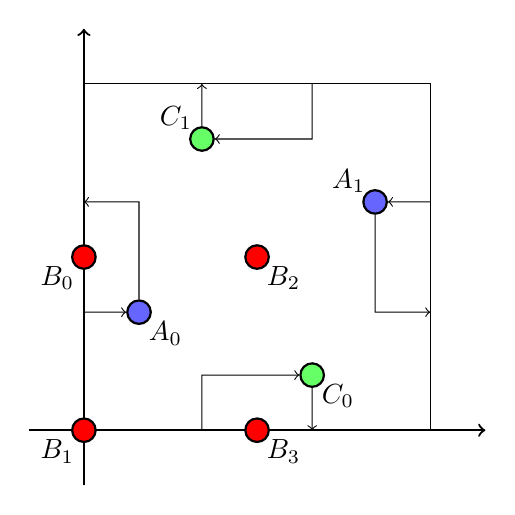
\begin{tikzpicture}[scale=0.7, vertex/.style={draw,circle,thick,fill=red,inner sep=3pt}]
\draw[->,thick] (-1,0) -- (2*pi+1,0);
\draw[->,thick] (0,-1) -- (0,2*pi+1);
\draw (0,0) rectangle (2*pi,2*pi);

\draw (0,0) node[vertex] {} node[below left] {$B_1$};
\draw (0,pi) node[vertex] {} node[below left] {$B_0$};
\draw (pi,0) node[vertex] {} node[below right] {$B_3$};
\draw (pi,pi) node[vertex] {} node[below right] {$B_2$};

\node[vertex,fill=blue!60] (A0) at (1,pi-1) {};
\node[vertex,fill=blue!60] (A1) at (2*pi-1,pi+1) {};
\draw[->] (0,pi-1) -- (A0);
\draw[->] (A0) node[below right] {$A_0$} -- (1,pi+1) -- (0,pi+1);
\draw[->] (2*pi,pi+1) -- (A1);
\draw[->] (A1) node[above left] {$A_1$} -- (2*pi-1,pi-1) -- (2*pi,pi-1);

\node[vertex,fill=green!60] (C0) at (pi+1,1) {};
\node[vertex,fill=green!60] (C1) at (pi-1,2*pi-1) {};
\draw[->] (C0) -- (pi+1,0);
\draw[->] (pi-1,0) -- (pi-1,1) -- (C0) node[below right] {$C_0$};
\draw[->] (C1) -- (pi-1,2*pi);
\draw[->] (pi+1,2*pi) -- (pi+1,2*pi-1) -- (C1) node[above left] {$C_1$};
\end{tikzpicture}
\caption{The contractible $4a$-periodic orbits of $H_1$ ($a > 2$), labeled. The label of an orbit is next to its starting point. For the non-constant orbits, the arrow represents the time-$2a$ flow.}
\label{orbitsh12}
\end{figure}

\subsection{Their Actions}

We now compute the actions of the orbits $A_0$, $A_1$, $B_0, \dots, B_3, C_0$ and $C_1$.

We begin with the constant orbits $B_i$. By a similar argument as the one done for the case of the Hamiltonian diffeomorphism $\phi$, the action of these orbits is simply the integral of $H_1$, which is given by $2a(\cos(y) - \cos(x))$. This concludes the computation of the action spectrum for $a < 2$.

Let us now inspect the orbits $A_i$ and $C_i$. Note that the paths these orbits take are squares, and therefore we may consider the embedded disk $D$ in the definition of the action functional to be a diffeomorphism between the interior of the disk and these squares. Furthermore, since the symplectic form $\omega$ is the area form on the torus, it pulls back to the area form on the square. Consequently, the $- \int_D \omega$ term in the action functional will be equal to the area of the square or its symmetric, depending on the orientation of the border: In the counterclockwise case ($A_0$, $A_1$) the orientation is positive, while in the clockwise case ($C_0$, $C_1$) it is negative. Finally, the area of these squares, in absolute value, is equal to their side squared, i.e. $(2x_0)^2 = 4x_0^2$.

Now we inspect the $\int H_1$ term in the action functional applied to these orbits. For the sake of concreteness, we will compute it for $A_0$, but the same argument goes for the other three.

The orbit $A_0$ can be divided into four (reparametrized) linear segments. For example, the first segment goes from $(x_0, y_0)$ to $(x_0, y_0 + 2a \sin(x_0)) = (x_0, \pi + x_0)$. Over this segment, the Hamiltonian $H_1$ takes the value $- \varphi(t) \cos(x_0)$ at time $t$, (see equation \eqref{h1def}) and integrating we obtain a contribution of $- a \cos(x_0)$ to $\int H_1$. It is easy to compute the contributions of the four other line segments. They are all also equal to $- a \cos(x_0)$, and so we conclude
\begin{equation}
\AA(A_0) = - 4 x_0^2 - 4 a \cos(x_0).
\end{equation}

It is easy to check that this value coincides with $\AA(A_1)$, and furthermore that
\begin{equation}
\AA(C_0) = \AA(C_1) = - \AA(A_0).
\end{equation}

As a last remark, we prove a simple inequality regarding $\AA(A_0)$, so that we can place the actions we have calculated so far on a line.

\begin{prop}\label{prop:ineq4beta}
Let $2 < a < \pi$ and $x_0$ be as in proposition \ref{prop:orbitsphi2}. Then, we have the inequality
\begin{equation}
0 < 4 x_0^2 + 4 a \cos(x_0) < 4a.
\end{equation}
\end{prop}

\begin{proof}
Since $0 < x_0 < \pi$, it should be obvious that $4 x_0^2 + 4 a \cos(x_0) > 0$, as it is a sum of two positive terms. Therefore, we turn to proving the other inequality.

Recall that $x_0$ satisfies the equality $x_0 = \frac a 2 \sin(x_0)$. Consequently, $4 x_0^2 = a^2 \sin^2 (x_0) = a^2 - a^2 \cos^2(x_0)$. Therefore,
\begin{equation}
4 x_0^2 + 4 a \cos(x_0) = a^2 + 4 a \cos(x_0) - a^2 \cos^2(x_0).
\end{equation}

Therefore, to show that $4 x_0^2 + a \cos(x_0) < 4a$ it suffices to show
\begin{equation}\label{eq:ineq4beta}
\begin{aligned}
&& a^2 + 4 a \cos(x_0) - a^2 \cos^2(x_0) &< 4a\\
\iff&& 4 (\cos(x_0)-1) + a(1 - \cos^2(x_0)) &< 0\\
\iff&& (\cos(x_0) - 1)(4 - a(1 + \cos(x_0))) &< 0\\
\iff&& 4 - a(1+ \cos(x_0)) &> 0\\
\iff&& a + a \cos(x_0) &< 4.
\end{aligned}
\end{equation}

The proof of this last inequality is somewhat involved. We begin by writing $a$ as a function of $x_0$, as
\begin{equation}
a = \frac{2 x_0}{\sin(x_0)}.
\end{equation}

Therefore, we intend to show that, for $x_0$ in, say, $\interval 0 {\frac \pi 2}$, the expression $\frac{x_0}{\sin(x_0)}(1 + \cos(x_0))$ is always less than 2. To this effect, we study the function
\begin{equation}
f(t) = \frac{t}{\sin(t)}(1 + \cos(t)).
\end{equation}

Laborious but straightforward computations will show that the derivative of $f$ is given by
\begin{equation}
f'(t) = - \frac{t - \sin(t)}{1 - \cos(t)}.
\end{equation}

Evidently, for $t > 0$, $f'(t) < 0$ where defined. Consequently, $f$ is a strictly decreasing function. Since $\lim_{t \to 0^+} f(t) = 2$, we obtain that $f(t) < 2$ for $t \in \ointerval 0 {\frac \pi 2}$, which completes the proof.
\end{proof}

We can now place the actions of the orbits on the real line, see figure \ref{actionsh12}.

\begin{figure}
\centering
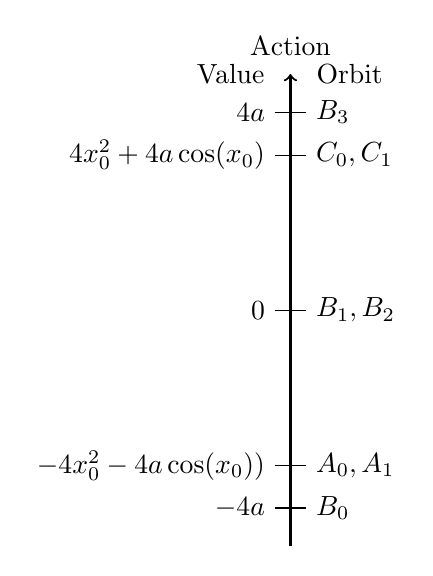
\begin{tikzpicture}[scale=0.2, tick/.style={left=0.2cm}, value/.style={right=0.2cm}]
\draw[->,thick] (0, -15) -- (0,15) node[above=0.1cm] {Action} node[tick] {Value} node[value]{Orbit};

\foreach \x in {-12.56,-9.85,0,9.85,12.56}
\draw (-1, \x) -- (1,\x);

\draw (0,-12.56) node[tick] {$-4a$} node[value] {$B_0$};
\draw (0,-9.85) node[tick] {$-4x_0^2 - 4 a \cos(x_0))$} node[value] {$A_0, A_1$};
\draw (0,0) node[tick] {$0$} node[value] {$B_1, B_2$};
\draw (0,9.85) node[tick] {$4x_0^2 + 4 a \cos(x_0)$} node[value] {$C_0, C_1$};
\draw (0,12.56) node[tick] {$4a$} node[value]  {$B_3$};


\end{tikzpicture}
\caption{The actions of the contractible periodic orbits of $H_1$ in time $4a$. The figure is to scale, with $a = 3.14$. As $a$ gets closer to $2$, the value of $4x_0^2 + 4a \cos(x_0)$ gets closer to $4a$.}
\label{actionsh12}
\end{figure}

\subsection{Their Maslov Indices}

We will now use corollary \ref{calcmaslov1} to compute the Maslov indices of the contractible orbits calculated above.

We begin with the orbits $B_0, \dots, B_3$, which are present for all $a > 0$. On these, the derivative can be calculated in a way similar to the computations in page \pageref{rectpath1}. Using the same notation as therein to represent piecewise rectilinear paths, the derivative matrix $A(t)$ at each $B_i$ is given by
\begin{equation}
\begin{multlined}
A(t):
\begin{bmatrix}
1 & 0\\
0 & 1
\end{bmatrix}
\to
\begin{bmatrix}
1 & 0\\
\pm_1 a & 1
\end{bmatrix}
\to
\begin{bmatrix}
1 \pm_1 \pm_2 a^2 &  \pm_2 a\\
\pm_1 a & 1
\end{bmatrix}\\
\to
\begin{bmatrix}
1 \pm_1 \pm_2 a^2 &  \pm_2 a\\
\pm_1 2a \pm_2 a^3 & 1 \pm_1 \pm_2 a^2
\end{bmatrix}
\to
\begin{bmatrix}
1 \pm_1 \pm_2 3 a^2 + a^4 &  \pm_2 2 a \pm_1 a^3\\
\pm_1 2a \pm_2 a^3 & 1 \pm_1 \pm_2 a^2
\end{bmatrix},
\end{multlined}
\end{equation}
where $\pm_1 1 = \cos(x)$ and $\pm_2 1 = \cos(y)$. We may now compute the trace of $A(t)$:
\begin{equation}
\trace A(t): 2 \to 2 \to 2 \pm_1 \pm_2 a^2 \to 2 \pm_1 \pm_2 2 a^2 \to 2 \pm_1 \pm_2 4 a^2 + a^4.
\end{equation}

We may remove the superfluous middle node, obtaining the equivalent representation
\begin{equation}\label{tracebi}
\trace A(t): 2 \to 2 \to 2 \pm_1 \pm_2 2 a^2 \to 2 \pm_1 \pm_2 4 a^2 + a^4.
\end{equation}

\begin{prop}
The Maslov indices of $B_1$ and $B_2$ are null.
\end{prop}

\begin{proof}
In this case, using the notation of equation \eqref{tracebi}, $\pm_1 = \pm_2$ and therefore the trace is always greater than or equal to two. Per corollary \ref{calcmaslov1}, this implies that the Maslov index is null.
\end{proof}

\begin{prop}
If $a < 2$, the Maslov indices of $B_0$ and $B_3$ are $-1$ and $1$ respectively. If $a > 2$, they are $-2$ and $2$.
\end{prop}

\begin{proof}
In this case, $\pm_1 \neq \pm_2$, and therefore the trace follows the path
\begin{equation}
\trace A(t) : 2 \to 2 \to 2 - 2a^2 \to 2 - 4a^2 + a^4.
\end{equation}

If $a<2$ then the trace starts at $2$, decreases, and doesn't reach $2$ again, as $2 - 4a^2 + a^4 = 2 - a^2 (a^2 - 4) < 2$. Therefore, we consider the partition $a_0 = 0$, $b_0 = 2a$, which is in the conditions of corollary \ref{calcmaslov1}, and so, for $a<2$,
\begin{equation}
\mu(A(t)) = \sign(A(2a)_{12}) = \sign(\pm_2 a) = \pm_2 1,
\end{equation}
which is what we wanted to prove.

\smallskip

We now consider the case $a > 2$. In this case the trace starts at 2, decreases to less than $-2$ and goes back up to more than 2 again. Therefore, our partition will now be of the form $a_0 < b_0 < a_1 < b_1$.

We set $a_0 = 0$ and $a_1 = 2a$. We define $b_0 = a(1+\varepsilon)$ for some small $\varepsilon$, in which case $\sign(A(b_0)_{12}) = \pm_2 1$.

The choice for $b_1$ is a bit trickier. We define $b_1$ in order to make the trace of $A(t)$ equal to zero, i.e., $b_1 = a(3 + t_0)$, where $t_0$ satisfies
\begin{equation}
2 - 2a^2 + (-2a^2 + a^4)t_0 = 0 \iff t_0 = \frac{2a^2 - 2}{a^4 - 2a^2}.
\end{equation}
Note: We don't need to verify that this expression is in $\interval 0 1$: it must be because $t_0$ was defined as the root of a linear function, which is known to be less than $-2$ at zero and greater than $2$ at one.

We can now compute $A(b_1)_{12}$ explicitly as
\begin{equation}
\pm_2 a \pm_2 (a - a^3) t_0 = \mp_2 \frac{2 + a^2(a^2 - 2)}{a(a^2 - 2)}.
\end{equation}

Given that $a^2 > 4 > 2$, the right-hand side has sign equal to $\mp_2$. In other words, $\sign(A(b_1)) = \mp_2 1$, and so, applying corollary \ref{calcmaslov1} we obtain
\begin{equation}
\mu(A(t)) = \pm_2 2.
\end{equation}

This completes the proof.
\end{proof}

We now turn to computing the Maslov indices of $A_1$, $A_2$, $C_1$ and $C_2$. To this effect, we begin by computing $(\dl \phi_t)_{(x_0,y_0)}$, in order to calculate the Maslov index of $A_1$.

Recall equation \eqref{rectpath}, which describes the path $A(t) = (\dl \phi_t)_{(x,y)}$ up to time $2a$
\begin{equation}\label{rectpath}
A(t) :
\begin{bmatrix}
1 & 0\\
0 & 1
\end{bmatrix}
\to
\begin{bmatrix}
1 & 0\\
a \cos(x) & 1
\end{bmatrix}
\to
\begin{bmatrix}
\scalebox{0.7}{$1+ a^2 \cos(y+a \sin(x)) \cos(x)$} &  a \cos(y)\\
a \cos(x) & 1
\end{bmatrix}.
\end{equation}

We plug in $(x,y) = (x_0, y_0)$. To simplify the expressions, we set $\beta = a \cos(x_0)$, to obtain
\begin{equation}
A(t) :
\begin{bmatrix}
1 & 0\\
0 & 1
\end{bmatrix}
\to
\begin{bmatrix}
1 & 0\\
\beta & 1
\end{bmatrix}
\to
\begin{bmatrix}
1 - \beta^2 &  -\beta \\
\beta & 1
\end{bmatrix}, t \in \interval 0 {2a}.
\end{equation}

Note that if we set $(x,y) = (-x_0, -y_0)$ we obtain the same expression. Furthermore, we have seen that $\phi(x_0, y_0) = (-x_0, -y_0)$, so that 1. the expression for $A(t)$ is the same if we start at $(-x_0, -y_0)$ and 2. by the chain rule we may write
\begin{equation}
A(2a + t) = A(2a) A(t), t \in \interval 0 {2a}.
\end{equation}

Therefore, the expression for $A(t)$ for $t \in \interval 0 {4a}$, associated to the paths $A_0$ and $A_1$, is given by
\begin{equation}
\begin{multlined}
A(t) :
\begin{bmatrix}
1 & 0\\
0 & 1
\end{bmatrix}
\to
\begin{bmatrix}
1 & 0\\
\beta & 1
\end{bmatrix}
\to
\begin{bmatrix}
1 - \beta^2 &  -\beta \\
\beta & 1
\end{bmatrix}\\
\to
\begin{bmatrix}
1 - \beta^2 &  -\beta \\
2 \beta - \beta^3 & 1 - \beta^2
\end{bmatrix}
\to
\begin{bmatrix}
1 - 3 \beta^2 + \beta^4 &  -2 \beta + \beta^3 \\
2 \beta - \beta^3 & 1 - \beta^2
\end{bmatrix}.
\end{multlined}
\end{equation}

Therefore, the trace of $A(t)$ follows the path
\begin{equation}
\trace A(t) : 2 \to 2 \to 2 - 2\beta^2 \to 2 - 4 \beta^2 + \beta^4,
\end{equation}
where the nodes are respectively at $0$, $a$, $3a$ and $4a$. The following proposition helps us describe qualitatively the behavior of the trace.

\begin{prop}
Using the notation $\beta = a \cos(x_0)$, we have the inequalities
\begin{align}
\label{beta1} 0 < \beta^2 &< 4\\
\label{beta2} -2 < 2 - \beta^2 &< 2,\\
\label{beta3} 2-2\beta^2 &< 2\\
\label{beta4} 2 - 4 \beta^2 + \beta^4 &< 2.
\end{align}
\end{prop}

\begin{proof}
We begin by proving \eqref{beta1}. The inequality $\beta^2 > 0$ is obvious from the fact that $\beta \neq 0$, as $0 < x_0 < \frac\pi2$. For the inequality $\beta^2 < 4$ we use the fact, which we proved in the middle of proving proposition \ref{eq:ineq4beta} (see equation \eqref{eq:ineq4beta0} that
\begin{equation}
\beta < 4 - a,
\end{equation}
and using the fact that $a > 2$ we immediately obtain $\beta < 2$ and hence $\beta^2 < 4$. This proves \eqref{beta1}.

Inequality \eqref{beta2} is obvious from \eqref{beta1}, and \eqref{beta3} is also obvious using $2 - 2 \beta^2 < 2 - \beta^2$. Finally, to prove \eqref{beta4} we use the factorization
\begin{equation}
2 - 4 \beta^2 + \beta^4 = 2 + \beta^2 (\beta^2 - 4).
\end{equation}

Since $\beta^2$ is positive and $\beta^2 - 4$ is negative, we obtain the desired inequality.
\end{proof}

\begin{corollary}
Let $A(t)$ be the matrix path given by the derivative of the flow of $H_0$ in the orbits $A_0$ and $A_1$. Then, the trace of $A(t)$ starts at 2, followed by a decrease, after which it always stays strictly below 2. Furthermore, at time $2a$ the trace, which equals $2 - \beta^2$, is in $\ointerval{-2}2$.
\end{corollary}

We are now able to compute the Conley-Zehnder index of $A(t)$, and consequently the Maslov indices of $A_0$ and $A_1$. We apply corollary \ref{calcmaslov1}, using the partition $a_0 = 0$ and $b_0 = 2a$. The conditions of this corollary are verified, and hence
\begin{equation}
\mu(A(t)) = \sign(-\beta) = -1,
\end{equation}
because $\beta$ is positive. Therefore,

\begin{prop}
The Maslov index of $A_0$ and $A_1$ is $-1$.
\end{prop}

The same computations apply almost without change for the orbits $C_0$ and $C_1$. The main difference is that $A(t)$ now becomes
\begin{equation}
\begin{multlined}
A(t) :
\begin{bmatrix}
1 & 0\\
0 & 1
\end{bmatrix}
\to
\begin{bmatrix}
1 & 0\\
-\beta & 1
\end{bmatrix}
\to
\begin{bmatrix}
1 - \beta^2 &  \beta \\
-\beta & 1
\end{bmatrix}\\
\to
\begin{bmatrix}
1 - \beta^2 &  \beta \\
-2 \beta + \beta^3 & 1 - \beta^2
\end{bmatrix}
\to
\begin{bmatrix}
1 - 3 \beta^2 + \beta^4 &  2 \beta - \beta^3 \\
-2 \beta + \beta^3 & 1 - \beta^2
\end{bmatrix},
\end{multlined}
\end{equation}
that is, the signs of the non-diagonal elements have been swapped. This preserves the trace and so the application of corollary \ref{calcmaslov1}, except that the term $\sign(-\beta)$ now becomes $\sign(\beta) = 1$. Consequently,

\begin{prop}
The Maslov index of $C_0$ and $C_1$ is 1.
\end{prop}

\begin{corollary}
The vector spaces of the filtered Floer complex of $H_1$ in time $4a$ are given by the following labeled barcodes. Figure \ref{bch1lt2} denotes the case where $0<a<2$ and figure \ref{bch1gt2} denotes the case $2<a<\pi$.

\begin{figure}[H]
\centering
\begin{tikzpicture}
\draw[->,thick] (-5.200,0.000)--(5.200,0.000);
\draw[] (0.000,-0.200)--(0.000,0.200) node[above] {0};
\draw[] (-3.200,-0.200)--(-3.200,0.200) node[above] {$-4a$};
\draw[] (3.200,-0.200)--(3.200,0.200) node[above] {$4a$};
\draw[(-,thick] (-3.200,-0.500)--(4.900,-0.500) node[right] {$B_0$};
\node[] at (6.200,-0.500) {$(\CF_{-1})$};
\draw[(-,thick] (0.000,-1.100)--(4.900,-1.100) node[right] {$B_1$};
\draw[(-,thick] (0.000,-1.500)--(4.900,-1.500) node[right] {$B_2$};
\node[] at (6.200,-1.300) {$(\CF_0)$};
\draw[(-,thick] (3.200,-2.100)--(4.900,-2.100) node[right] {$B_3$};
\node[] at (6.200,-2.100) {$(\CF_{1})$};
\end{tikzpicture}
\caption{The barcode of the filtered Floer complex of $H_1$ in time $4a$, for $0<a<2$}\label{bch1lt2}
\end{figure}

\begin{figure}[H]
\centering
\begin{tikzpicture}[scale=0.35]
\draw[->,thick] (-13.766,0.000)--(13.766,0.000);
\draw[] (0.000,-0.200)--(0.000,0.200) node[above] {0};
\draw[] (-12.566,-0.200)--(-12.566,0.200) node[above] {$-4a$};
\draw[] (12.566,-0.200)--(12.566,0.200) node[above] {$4a$};
\draw[] (-8.870,-0.200)--(-8.870,0.200) node[above] {$-4 x_0^2 - 4 \beta$};
\draw[] (8.870,-0.200)--(8.870,0.200) node[above] {$4 x_0^2 + 4 \beta$};
\draw[(-,thick] (-12.566,-1.200)--(13.586,-1.200) node[right] {$B_0$};
\node[] at (16.766,-1.200) {$(\CF_{-2})$};
\draw[(-,thick] (-8.870,-2.550)--(13.586,-2.550) node[right] {$A_0$};
\draw[(-,thick] (-8.870,-3.750)--(13.586,-3.750) node[right] {$A_1$};
\node[] at (16.766,-3.150) {$(\CF_{-1})$};
\draw[(-,thick] (0.000,-5.100)--(13.586,-5.100) node[right] {$B_1$};
\draw[(-,thick] (0.000,-6.300)--(13.586,-6.300) node[right] {$B_2$};
\node[] at (16.766,-5.700) {$(\CF_0)$};
\draw[(-,thick] (8.870,-7.650)--(13.586,-7.650) node[right] {$C_0$};
\draw[(-,thick] (8.870,-8.850)--(13.586,-8.850) node[right] {$C_1$};
\node[] at (16.766,-8.250) {$(\CF_{1})$};
\draw[(-,thick] (12.566,-10.200)--(13.586,-10.200) node[right] {$B_3$};
\node[] at (16.766,-10.200) {$(\CF_{2})$};
\end{tikzpicture}
\caption{The barcode of the filtered Floer complex of $H_1$ in time $4a$, for $2 < a < \pi$}\label{bch1gt2}
\end{figure}
\end{corollary}

\subsection{The Boundary Maps}

We now turn to computing the boundary maps of the filtered Floer complex of $H_1$ in time $4a$, for $2 < a < \pi$, using symmetries and the fact that Floer homology coincides with Morse homology. Strictly speaking, the latter is sufficient to compute the barcode of $H_1$, albeit not the boundary maps themselves. The method of symmetries allows us to obtain more details.

We recall the method of symmetries, explained in \ref{sec:symmetries}. If we let $\partial(b) = \sum n(b,c) c$, the scalar $n(b,c)$ can be computed by counting the number of pseudo-holomorphic curves (see the differential equation \eqref{pseudoholomorphic}) which connect $b$ and $c$ in the $C^\infty$ sense. The idea in \ref{sec:symmetries} is that if we find a change of variables which preserves the orbits $b$ and $c$, as well as the equation for pseudo-holomorphicity, we can draw conclusions about $n(b,c)$. In this case, we will soon modify the method slightly: Our symmetries may now not preserve $b$ and $c$, and instead we will find relations between, say, $n(b,c)$ and some other $n(b', c')$.

We begin by applying the method to compute $n(B_i, A_j)$ for $i = 1, 2$, $j = 0, 1$. We consider the change of variables
\begin{equation}
x \to -x, y \to y, t \to 3a - t.
\end{equation}

It is straight-forward to check that this change of variables preserves $A_j$ and $B_2$, and the verifications done in section \ref{sec:symmetries} suffice to show that it preserves pseudo-holomorphicity. Therefore, by the same argument done therein, applied to $t = \frac32 a$, we obtain that $n(B_2, A_j) = 0 \mod 2$. The same argument, swapping the sign of $y$ instead of $x$ and setting $t \to a - t$ instead, suffices to show $n(B_1, A_j) = 0$.

These same symmetries can be used to show that $n(C_i, B_j) = 0$, for $i = 0, 1$ and $j = 1, 2$, and so we conclude
\begin{prop}\label{fch14a1}
The filtered Floer complex of $H_1$ in time $4a$ is of the form
\begin{equation}
\dots \leftarrow 0 \leftarrow \CF_{-2}^\lambda \xleftarrow{\partial} \CF_{-1}^\lambda \xleftarrow{0} \CF_0^\lambda \xleftarrow{0} \CF_1^\lambda \xleftarrow{\partial} \CF_2^\lambda \leftarrow 0 \leftarrow \dots
\end{equation}
\end{prop}

Again, we remark that the information that the Floer homology coincides with Morse homology would have sufficed to prove proposition \ref{fch14a1} and also compute the rank of the remaining boundary maps, which is enough to compute the barcode of $H_1$. However, symmetries give us a little bit more detail.

\begin{prop}\label{fch14a2}
The border maps in proposition \ref{fch14a1} are non-null, and satisfy
\begin{equation}\label{eq:partialsh1}
\begin{gathered}
\partial(A_0) = \partial(A_1) = B_0,\\
\partial(B_3) = C_0 + C_1.
\end{gathered}
\end{equation}
\end{prop}

\begin{proof}
The fact that the border maps are non-null stems from the fact that Floer homology coincides with Morse homology (up to a shift by one of the index). For example, if $\partial(B_3) = 0$ then $B_3$ would be in the kernel of $\partial \colon \CF_2 \to \CF_1$, and since $\CF_3$ is null, we would have $\HF_2(H_1) = \braket{B_3}$, which does not coincide with the third Morse homology of the torus, which is null. The argument for the other partial map is similar.

To show equation \eqref{eq:partialsh1}, simply use the change of the variables $t \to 2a + t$ to show $n(A_0,B_0) = n(A_1,B_0)$ and $n(B_3,C_0) = n(B_3,C_1)$.
\end{proof}

\subsection{Conclusion and Corollaries}

\begin{theorem}
Let $\phi(x,y)$ be the Hamiltonian diffeomorphism given by
\begin{equation}
\phi(x,y) = (x+a \sin( y + a \sin(x)), y + a \sin(x)).
\end{equation}

Then, for $0 < a < 2$, the barcode of $\phi^2$ is given by
\begin{figure}[H]
\centering
\begin{tikzpicture}
\draw[->,thick] (-5.200,0.000)--(5.200,0.000);
\draw[] (0.000,-0.200)--(0.000,0.200) node[above] {0};
\draw[] (-3.200,-0.200)--(-3.200,0.200) node[above] {$-4a$};
\draw[] (3.200,-0.200)--(3.200,0.200) node[above] {$4a$};
\draw[(-,thick] (-3.200,-0.500)--(4.900,-0.500);
\node[] at (6.200,-0.500) {$(\HF_{-1})$};
\draw[(-,thick] (0.000,-1.100)--(4.900,-1.100);
\draw[(-,thick] (0.000,-1.500)--(4.900,-1.500);
\node[] at (6.200,-1.300) {$(\HF_0)$};
\draw[(-,thick] (3.200,-2.100)--(4.900,-2.100);
\node[] at (6.200,-2.100) {$(\HF_{1})$};
\end{tikzpicture}
\caption{The barcode of the filtered Floer homology of $\phi^2$, for $0<a<2$.}
\end{figure}

For $a = 2$, $\phi^2$ is a degenerate Hamiltonian diffeomorphism.

For $2<a<\pi$, the barcode of $\phi^2$ is given by
\begin{figure}[H]
\centering
\begin{tikzpicture}[scale=0.33]
\draw[->,thick] (-14.066,0.000)--(14.066,0.000);
\draw[] (0.000,-0.200)--(0.000,0.200) node[above] {0};
\draw[] (-12.566,-0.200)--(-12.566,0.200) node[above] {$-4a$};
\draw[] (12.566,-0.200)--(12.566,0.200) node[above] {$4a$};
\draw[] (-8.870,-0.200)--(-8.870,0.200) node[above] {$-4 x_0^2 - 4 \beta$};
\draw[] (8.870,-0.200)--(8.870,0.200) node[above] {$4 x_0^2 + 4 \beta$};
\draw[{(-]},thick] (-12.566,-1.200)--(-8.870,-1.200) node[right] {};
\node[] at (17.066,-1.200) {$(\HF_{-2})$};
\draw[(-,thick] (-8.870,-2.700)--(13.841,-2.700) node[right] {};
\node[] at (17.066,-2.700) {$(\HF_{-1})$};
\draw[(-,thick] (0.000,-4.200)--(13.841,-4.200) node[right] {};
\draw[(-,thick] (0.000,-5.400)--(13.841,-5.400) node[right] {};
\node[] at (17.066,-4.800) {$(\HF_0)$};
\draw[(-,thick] (8.870,-6.900)--(13.841,-6.900) node[right] {};
\draw[{(-]},thick] (8.870,-8.100)--(12.566,-8.100) node[right] {};
\node[] at (17.066,-7.500) {$(\HF_{1})$};
\end{tikzpicture}
\caption{The barcode of the filtered Floer homology of $\phi^2$, for $2<a<\pi$.}
\end{figure}
\end{theorem}

\begin{corollary}
For $2 < a < \pi$, the Hamiltonian diffeomorphism $\phi$ is not generated by an autonomous Hamiltonian.
\end{corollary}

\begin{proof}
If $\phi$ were generated by an autonomous Hamiltonian, so would $\phi^2$ (as one could flow with the same Hamiltonian in twice the time). Therefore, it suffices to show that $\phi^2$ is not generated by an autonomous Hamiltonian.

Recall that (proposition \ref{maslovmorse}) the Maslov indices of critical points of a Hamiltonian diffeomorphism induced by an autonomous Hamiltonian are all zero or odd. Therefore, the barcode of such a diffeomorphism cannot have any bars in index $-2$, and every bar in index $1$ must only terminate at infinity. Neither of these conditions are satisfied by the barcode of $\phi^2$.

On a slightly more elementary level, the proof boils down to the fact that $\phi^2$ has fixed points ($B_0$ and $B_3$) with Maslov index $\pm 2$.
\end{proof}